\subsubsection{Heurística Constructiva Golosa}

\subsubsubsection{Medición en base a tamaño del grafo}
La complejidad de la heurística constructiva golosa es $\mathcal{O}(n * (log(n) + D))$, con lo cual se espera una curva que crezca a medida que se incrementa el valor de n.

\begin{figure}[H]
	\centering
	\begin{minipage}[t]{.45\textwidth}
		\centering
		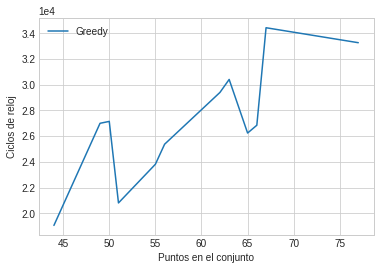
\includegraphics[scale=0.55]{exercise5/greedy3}
	\end{minipage}\qquad
	\begin{minipage}[t]{.45\textwidth}
		\centering
		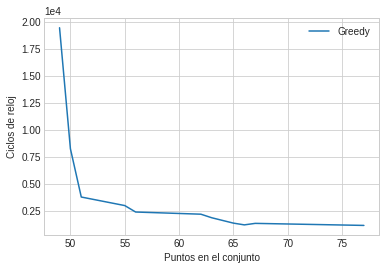
\includegraphics[scale=0.55]{exercise5/greedyAcotado}
	\end{minipage}
\end{figure}

El resultado obtenido es similar al esperado ya que se pueden detectar casos en los que la ejecución es más rápida que puntos anteriores. Sin embargo, la curva luego vuelve a crecer, consistentemente con nuestra suposición. El gráfico del lado derecha representa los valores usados para el gráfico de la izquierda divididos por una la cota de complejidad temporal. Al ver que el gráfico converge, podemos concluir que la heurística respeta la complejidad temporal planteada.

Los casos de resoluciones rápidas podrían deberse a juegos de datos que favorecen a la heurística.


\subsubsubsection{Medición en base a distribución del grafo}


En este caso, se utilizó una instancia en la que los nodos de mayor demanda se encontraban cerca del depósito contra una en la que no. Se espera entonces que la diferencia de tiempos entre los juegos de datos sea grande.

\begin{figure}[H]
	\centering
	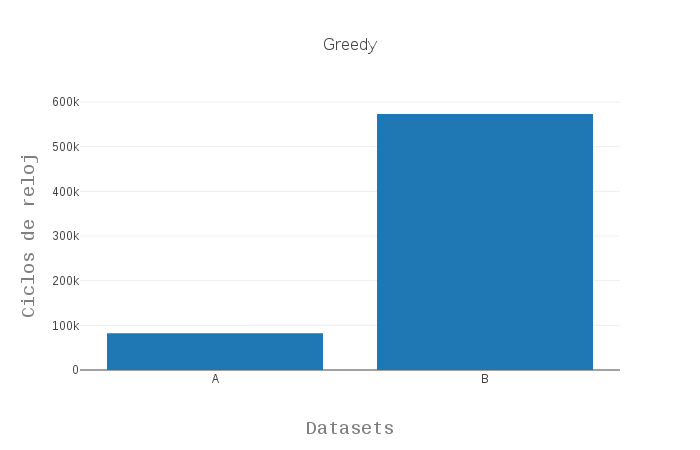
\includegraphics[scale=0.4]{exercise5/greedyType.png}
\end{figure}


Tal como se esperaba, el caso en el que los nodos de mayor demanda se encontraban más cerca del depósito se resuelve más rápidamente. Esto es porque en su ejecución, el algoritmo ordena los puntos por demanda y luego cercanía al depósito.